\documentclass[12pt]{article}
\usepackage{hyperref}
\usepackage{amsmath}

\usepackage{tikz}
\usetikzlibrary{shapes,arrows}

\tikzstyle{block} = [draw, fill=blue!20, rectangle, 
    minimum height=2em, minimum width=5em]
\tikzstyle{input} = [coordinate]
\tikzstyle{output} = [coordinate]

\title{Report on Language Modeling.}
\author{Alistair Valentin (ab667)\\
\and Alec Sullivan (ajs394)\\
\and Hee Jung Ryu (hr99)\\
\and Matthew Lepage (mcl82)\\
\and Saeed Abdullah (sma249)}
\date \today




\begin{document}
\maketitle

Our submission, written in the language Python, reads in raw text, cleans and formats it with the help of NLTK, and generates a smoothed and efficient dictionary of both N-grams for perplexity-based text similarity calculation and (N-1)-grams for sentence generation.

To summarize, in this report, we discuss about
\begin{itemize}
\item Our implementation of unigram and bigram from Dataset1 and Dataset2.
\item Handling unknown words (trivial).
\item The implementation of Laplace smoothing.
\item The design and functionality of random sentence generator.
\item Design of email author prediction and the analysis of result.
\item Implementation of a general N-gram model (extension 1).
\item Design and implementation of Simple Good Turing smoothing (extension 2)
\item Nontrivial handling unknown words (extension 4).
\end{itemize}
\section{Preprocessing}

For text normalization, we first use sentence segmentation to mark the boundary
of the sentences and then perform lemmatization and word tokenization.

\begin{center}
\begin{figure}[!htb]
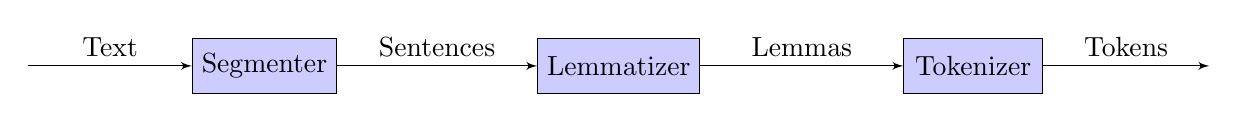
\begin{tikzpicture}[auto, node distance=4.5cm,>=latex']

\node [input, name=input] {};
\node [block, right of=input, node distance=3cm] (segmenter) {Segmenter};
\node [block, right of=segmenter] (lemmataizer) {Lemmatizer};
\node [block, right of=lemmataizer] (tokenizer) {Tokenizer};
\node [output, right of=tokenizer, node distance=3cm] (output) {};
\draw [->] (segmenter) -- node[name=u] {Sentences} (lemmataizer);
\draw [->] (lemmataizer) -- node {Lemmas} (tokenizer);
\draw [->] (tokenizer) -- node{Tokens} (output);
\draw [->] (input) -- node{Text} (segmenter);

\end{tikzpicture}
\caption{\label{fig:preprocess} Steps in Text Preprocessing.}
\end{figure}
\end{center}


\subsection{Sentence Segmentation}
Initially we used period to mark the boundary of sentence, but period
simultaneously indicate the termination of sentence and abbreviation. For
example, using period as boundary indicator does not work for 
the sentence \texttt{Mr. A got his Ph.D. from U.S.A.}, so to divide the
text into individual sentences we use Punkt sentence segmenter
\cite{kiss2006unsupervised} from NLTK.

\subsection{Lemmatization}
For grouping different inflicted forms of a word into a single term, we use
WordNet lemmatizer from NLTK. After applying lemmatizer on each sentences
from previous step, we get a sequence of lemma.

\subsection{Tokenization}
To split the sentence into words and punctuation, we use
TreebankWordToeknizer from NLTK. It tokenizes using the conventions from Penn
Treebank\footnote{http://www.cis.upenn.edu/~treebank/tokenization.html}.
Contractions are split into their component morphemes. For example,
\texttt{You're} are split into \texttt{You} and \texttt{'re}.

The implementation of the preprocessing is in
\href{https://github.com/saeed-abdullah/cs4740-language-model/blob/master/languagemodel/util.py\#L5}
{util.py}. After processing the given file, the output file contains
one sentence per line where each sentence consists of words and punctuation
separated by a single space.

\section{N-Gram generation}
In stead of handling unigram, bigram, trigram and so on as separate cases, we
use a more generalized approach to handle N-grams in our
\href{https://github.com/saeed-abdullah/cs4740-language-model/blob/master/languagemodel/NGrams.py}
{code}. To do so, we use the fact that for any calculation, we only need to keep
track of frequency for N and N-1 grams --- $c(w_{n-N+1}^{n})$ and 
$c(w_{n-N+1}^{n-1})$, respectively.

So, for building n-gram based language models, we keep two dictionaries for
N and N-1 grams, where the keys are the ngrams and the values represents
the frequency of that ngram.

\section{Smoothing}

We \href{https://github.com/saeed-abdullah/cs4740-language-model/blob/master/languagemodel/probability.py}
{implemented} both Laplace and Good-Turing smoothing.
\subsection{Laplace smoothing}
For unigram, we calculated the Laplace smoothing as:
\[P_{\text{Laplace}}(w_i) = \frac{c_i + 1}{N + V},\]
where $V$ is the size of vocabulary and $N$ is the number of tokens
in the dataset.

For bigram, the Laplace smoothing is calculated as:
\[P_{\text{Laplace}}P(w_n|w_{n-1}) = 
\frac{C(w_{n-1}w_n)  + 1}{C(w_{n-1}) + V}.\]

\subsection{Simple Good Turing smoothing}

For implementing Good-Turing smooth, we use the method from the original
paper from Gale and Samson \cite{gale1995good}. For smoothing curve,
they suggested using a power-curve:
\[N_r = a * r^b,\]
where $r$ is the frequency and $N_r$ is the frequency of frequency. For
estimating $a$ and $b$, we can plot $\log N_r$ and $\log r$, but as for
large $r$, the probability of $N_r$ being $0$ is high. So, we use plot
$\log Z_r$ and $\log r$, where
\[Z_r = \frac{N_r}{0.5 * (t-q)},\]
where $q$, $r$ and, $t$ are the indices of consecutive non-zero frequency
of frequency with $q < r < t$. When $r$ is $1$, $q$ is set to 0. For the
last index, $t = 2r - q$. Then, we use linear regression to determine $a, b$.

It is also suggested that a simple curve is more appropriate for higher $r$.
As Gale and Sampson \cite{gale1995good} proposes, we use $r$ while the
difference between $r$ and $r^{*}$ if it is 1.96 greater than the
standard deviation. So, we switch to $r*$ if:
\[ |r - r^*| \leq 1.96 \sqrt{(r+1)^2 \left(N_{r + 1} / N_{r}^{2}\right)
\left(\frac{1 + N_{r+1}}{N_r}\right)}\]


% From Hee
\section{Unknown Word handling}
\subsection{Trivial Unknown Word Handling}


As described in the text \cite{jurafskybook2009} our algorithm limits the ngram models’ vocabulary size by modifying the training corpus. The first 15 tokens in the training corpus are added to the unknown word list, and all future occurrences of these tokens in the corpus are replaced with the string ``UNK'', signifying their being unknown words. This approach is a simple and modular tweak that could be easily built into our existing N gram structure.

The number 15 was chosen after a few trials on the various training sets. As there were a lot of repeated tokens at the beginning of the corpora, choosing the first 15 tokens resulted in reasonable numbers of unique tokens to be treated being treated as unknowns. Smaller values caused very small unique unknown words (perhaps due to the heavy use of HTML tags in our data sets), and though this number may have to be adjusted for different data sets it works well for our given training corpus .



\section{Nontrivial Unknown Word Handling}

The basic approach of out nontrivial unknown word handling is the same for trivial handling, with the difference being that this algorithm keeps two unknown word lists: a trivial unknown word list of words replaced with ``UNK" and a nontrivial unknown word list for words replaced with ``UNKS\_NONTRIV". When a token from the first 15 tokens in the training corpus was comprised of only letters and contained at least one vowel and a consonant, the token is considered nontrivial and added to the second list. The rest of the first 15 tokens in the training corpus were considered to be trivial unknown words. Meaningful English words usually consist of only letters with at least one vowel and a consonant, so this criteria reflects this language trait. As above, this approach is especially applicable to our data set, with its large number of HTML syntax tags. Sentences was generated by our random sentence generator were surprisingly readable, which gives us faith in this approach

% From Alistair:
\section{Random Sentence Generator}
The random sentence generator works essentially by finding the set of all start sentences and picks one based upon the weighted probability of each start marker - the number of times that particular start marker appears over the number of total start markers. After choosing a start word, it adds that word to the sentence and continues looking for N-Grams that start with the next logical sequence of words from the previous N-Gram - i.e. it removes the first word of the N-Gram and searches for N-Grams that start with the words other than the first. It runs until the weighted choice chooses an N-Gram with the ``\_END\_" marker in it, at which point it ends the sentence creation and returns the completed sentence. Our data structures for storing N-grams allow for access to performing random sentence generation across general N-Grams, rather than just unigrams and bigrams.  

We build the random sentences for unigrams based upon the calculated probability of the number of times it appears in the corpus over the number of words and word types in the corpus. After choosing a start word, it then randomly chooses a word (the probability is weighted by the frequency of the word in the corpus) and continues until it selects an end marker.

The bigrams calculate the probability of the next bigram by $P(w2|w1) = \frac{\#(w1 w2)}{\#(w1)}$, i.e. the number of times a specific bigram appears over the total number of times the first word in the bigram appears. 

There is also the ability to build sentences from previously computed probabilities stored in Hash Tables, which is how we computed the example sentences below. This required a bit of re-factoring the initial code for computing random sentences, but the NGram object that we have constructed or precomputed tables of unigrams and bigrams with their respective frequencies are possibilities for creating random sentences. The keys and values were stored in JSON format which are then loaded into python for computing, and on large corpora this is where a significant amount of the processing time occurs, as it takes a fair amount of time to load a nearly 30MB JSON file. 

\subsection{Sample Unigram Randomly Generated Sentences:}
(Note that some words like was are truncated)

\begin{itemize}
\item \texttt{nation $>$ said at STREET The the state be the delivery 15 and 's offer York whether P=100 published having the of and HEADER the}

\item \texttt{13D $>$ group ( over Quesnot one the police illegal Hospital promote product Smith  Gouled a I are $>$ a reform this up want 's from annual of ] censured direct Rangoon F leading , $>$ the [ ,}

\item \texttt{market member attract network}

\item \texttt{began project of territory is general Chapter Reassessing possessed . is opposition $<$ exponentially in $>$ puppet F English appropriate -- well attended Texaco ended effort the the Academy $<$ early of $>$ it $>$ 200 wa Mass Tyrrell $<$ $>$ threatened Grenfell principle}

\item \texttt{of for wa revolutionary become KCNA /F a Mitchell two side If did ha illegal for country because investigation $<$ 1 on}
\end{itemize}


\subsection{Sample Bigram Randomly Generated Sentences:}

\begin{itemize}
\item \texttt{Recently , Even space agency traditionally an Lt-Gen Kitti Rattanachaya yesterday .}

\item \texttt{Mr. Babbitt declared my also voted yesterday , to an enterprise profit of price fell , but any 's support for ahead with RIA-Novosti may appear to good of the announcement that based on inspection and we were Louis Shill 's unemployment , nearly 3 , in arranging a Television Network in it Serial Products sector is controlled by Indian law saying : For Trade and Russia Federation : $<$ F in an file the result , argues vehemently denied some major drug .}

\item \texttt{Principal-only security , BOFT official fear they consume shifted to kill by the public surrounding area .}

\item \texttt{Premier Hong Kong EASTERN EXPRESS in to the will not be the military law would be the non- warrant .}

\end{itemize}

\section{Perplexity}

For perplexity, we take the logarithm value for better precision:

\begin{align*}
\log PP(W) &= \log \sqrt[N]{\prod_{i=1}^{N}\frac{1}{P(w_i | w_{i-1})}}\\
    &=-\frac{1}{N}\sum_{i=1}^{N}\log P(w_i | w_{i-1})
\end{align*}

For language modeling, we use the combined train sets from Dataset1 and
Dataset2 with Laplace smoothing.

\begin{table}[htb]
\begin{center}
\begin{tabular}{|c|c|c|}
\hline
&Dataset 1 & Dataset 2\\
\hline
unigram & $13.854$ & $13.155$\\
\hline
bigram & $11.9678$ & $11.1329$\\
\hline
\end{tabular}
\end{center}
\caption{\label{table:perplexity} Log Perplexity.}
\end{table}
From Table \ref{table:perplexity}, the perplexity across datasets seems
consistent. The perplexity is considerably low when using bigram comparing
to the language model built using unigram, as expected.


\section{Kaggle result}

\subsection{Implementation}
 We first segmented the validation and test corpora of emails into a set of individual emails with a corresponding author token. We then trained three separate n-gram models, one for each author, on the training data. For each email, we determined the perplexity of each n-gram was determined with respect to that email, and that email’s author was predicted as the n-gram with the lowest perplexity. These predictions were then output to a record file, to be iterated through and checked against our previously made email and author set.
\begin{table}[htb]
\begin{center}
\begin{tabular}{|c|c|}
\hline
\textbf{Dataset} & \textbf{Accuracy}\\
\hline
Validation Set & $80.24\%$\\
\hline
Test Set & $34.29\%$\\
\hline
Kaggel & $80.78\%$\\
\hline
\end{tabular}
\caption{\label{table:kaggle-result}Accuracy on different dataset.}
\end{center}
\end{table}


\subsection{Analysis}
While our algorithm was quite accurate on the validation set, it did not generalize well to the test set.  Since Kaggel only uses a selection from the test data, it stands to reason that the emails selected from test to be used by Kaggel were generally among the relatively small percentage that our algorithm predicted correctly.  It is interesting to note that our algorithm performed on the full test set only slightly better than it would have if it was randomly selecting between the three authors.  This perhaps means that there is a degree of over-fitting to the validation set causing a lack of flexibility, but judging by the number of other low scores on Kaggel from other groups it is also possible that performance on the test set was generally bad due to the relative author frequencies within it; the test set was entirely populated with emails written by the author for which there was the least training and validation data, so it makes sense that it would score better on the more diverse validation set.

\bibliography{bibinfo}
\bibliographystyle{plain}
\end{document}
